\chapter{Regulator}
\label{cha:regulator}

\section{Zaproponowany regulator}
\subsection{Regulator PID}
Do pozycjonowania manipulatora zaproponowany został regulator składający się z dwóch równolegle połączonych regulatorów PID. Kiedy trzymana jest pełna szklanka, to na wyjście przekazywane jest sterowanie z pierwszego regulatora, a kiedy jest pusta to z drugiego. Regulatorom postanowiono zadać inne nastawy, takie, by ograniczyć przyspieszenie kątowe w~sytuacji, gdy trzymana jest pełna szklanka.Ma to na celu spełnienie warunku, by przyspieszenie było małe, aby nie wylać wody. Struktura obu regulatorów jest identyczna, wyrażona następujący wzorem:
\begin{equation}\label{key}
U = (P + I \frac{1}{s} + D\frac{sN}{S+N}) E
\end{equation}
gdzie:\\
$
U$ - sterowanie\\
$E$ - uchyb regulacji\\
$P, I, D$ - współczynniki odpowiednio od części proporcjonalnej, całkującej i różniczkującej.\\
Na podstawie przeprowadzonych symulacji przyjęto następujące nastawy regulatorów:\\
Regulator odpowiedzialny za pozycjonowanie ramienia z napełnioną szklanką:\\
$
P = 3\\
I = 0.2\\\
D = 1.5\\
$\\
Regulator pozycjonujący ramie z pustą szklanką:\\
$
P = 3\\
I = 0.002\\
D = 1\\
$
Pozycja zadana podawana na regulator manipulatora miała postać funkcji prostokątnej. Stwierdzono jednak, że z uwagi na ograniczenie przyspieszenia, czas pozycji zadanej dla ruchu z pełną szklanką powinien być dłuższy. Na tej podstawie przyjęto czas pozycjonowania ramienia z napełnioną szklanką na 3~s, a czas powrotu ramienia na pozycję początkową na 2~s.\\
Na rysunku \ref{pid_res} przedstawiono odpowiedz układ dla opisanych powyżej regulatorów.
\begin{figure}[h!]
	\centering
	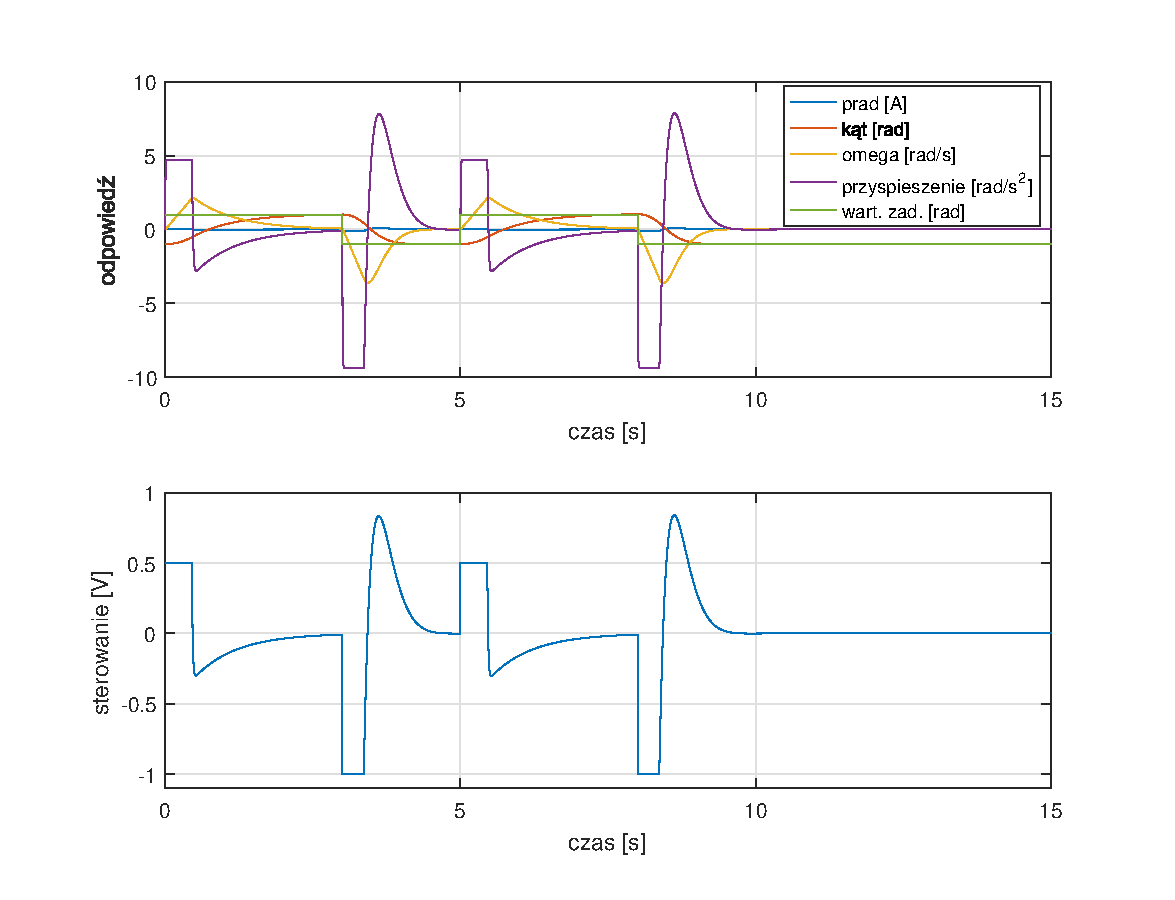
\includegraphics[scale = 0.9]{fig/pid_response.eps}
	\caption		
	{Wartości zmiennych stanu i sterowania.}
	\label{pid_res}
\end{figure} 
Dla tak przyjętych nastaw regulatorów otrzymano następujące wartości wska\'zników jakość:\\
$J_1 = 3.847 \ [rad^2 \cdot s]$\\
$J_2 = 0.7587 [V^2 \cdot s]$\\
$J_3 = 4.606$\\

\subsection{Regulator neuronowy}
Regulator neuronowy został zaprojektowany w ten sposób aby otrzymać analogiczne przebiegi sygnałów jak w przypadku klasycznego regulatora PID, wykorzystując do tego celu jeden neuron. Przyjęto, że wektor sygnałów wejściowych będzie miał następującą postać: 
\begin{equation}\label{key}
x = \begin{bmatrix}
\dot {e}\\
e\\
\int e\\
\dfrac{z-z_{min}}{z_{max} - z_{min}}\\
\end{bmatrix}
\end{equation}
gdzie:\\
$e$ - uchyb regulacji\\
$z$ - wart. zadana\\
$z_{min}, \ z_{max}$ - odpowiednio minimalna i maksymalna wart. zadana\\
Współczynnik skalujący z racji na to, że w rozważanym przypfdku wymagane są dwa regulatory jest w postaci macierzy: 
\begin{equation}\label{key}
W = \begin{bmatrix}
D_1& P_1& I_1&0\\
D_2& P_2& I_2&0\\
0&0&0&1
\end{bmatrix}
\end{equation} 
Stała składowa dla tak przyjętej postaci regulatora jest trójelementowym wektorem:
\begin{equation}\label{key}
b = \begin{bmatrix}
0\\0\\0
\end{bmatrix}
\end{equation}
Z racji na to że w zależności od tego czy przestawiamy pustą szklankę czy pełną należy zmieniać nastawy regulatora oraz saturację sygnału sterującego. Po uwzględnieniu tych wymagań przyjęto następującą postać funkcji:
\begin{equation}\label{key}
f(u,z) = f_{sat1} ((1-z) \cdot u_1 + z \cdot u_2) \cdot (1-z) + f_{sat2} ((1-z) \cdot u_1 + z \cdot u_2) \cdot z
\end{equation}
gdzie: \\
$z - $przeskalowania wartość zadana do przedziału [0,1]\\
$u_1, \ u_2 - $wartości sterowania odpowiednio od regulatorów dla pełnej i pustej szklanki.\\
$f_{sat1}, \ f_{sat2}$ - funkcje saturacji dla pełnej i pustej szklanki.
 \\
 Przeanalizowano dwie postaci funkcji saturacji: 
 \begin{enumerate}
 	\item klasyczna funkcja opisana równaniem :
 	\begin{equation}\label{sat_klas}
 	f_{sat}(x) = 
 	\begin{cases}
 	-K       & \quad x < y_{min}\\
 	x  & \quad x \in [y_min, \ y_max]\\
 	K       & \quad x > y_{max}\\
 	\end{cases}
 	\end{equation}
 	\item przybliżenie funkcją sigmoidalną postaci:
 	\begin{equation}\label{key}
 	f_{sat}(x) = (\dfrac{2}{1+\exp{-\beta \cdot x}} - 1) \cdot K
 	\end{equation}
 \end{enumerate}
gdzie:\\
$K$ - maksymalna dozwolona wartość sterowania podawanego na obiekt.\\
Parametry funkcji sigmoidlanych $\beta$ zostały dobrane za pomocą funkcji \textit{fmincon} tak aby zminimalizować różnice w stosunku do zależności opisanych równaniami \ref{sat_klas}.Finalnie otrzymano następujące wartości parametrów:\\
$\beta1 = -2.65$\\
$\beta2 = -5.33$\\

\begin{figure}[h!]
	\centering
	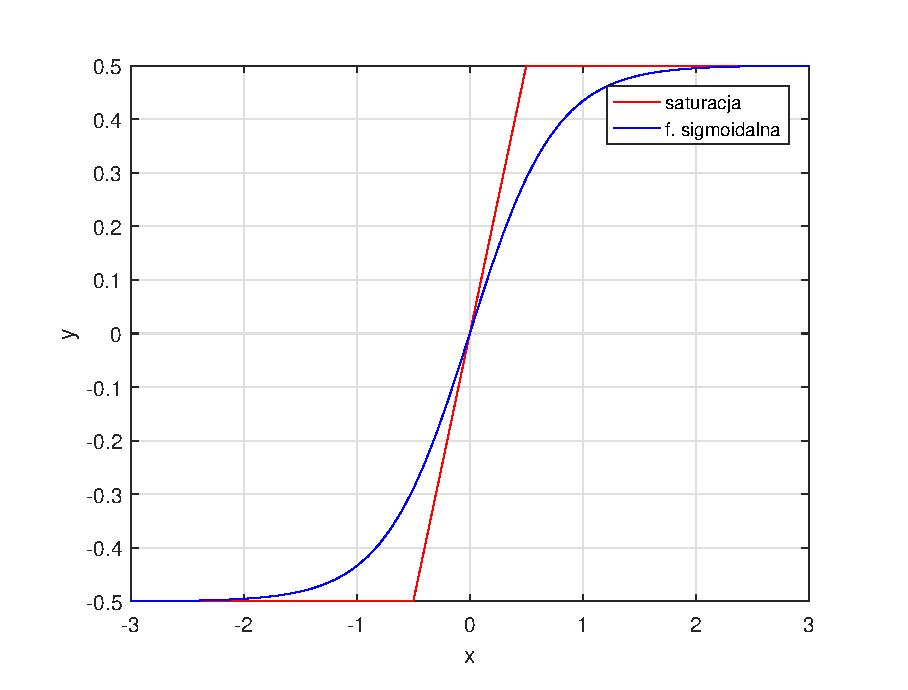
\includegraphics[scale = 0.8]{fig/por_sat_1.eps}
	\caption		
	{Porównanie saturacji i funkcji sigmoidalnej - pełna szklanka.}
	\label{por_sat1}
\end{figure} 

\begin{figure}[h!]
	\centering
	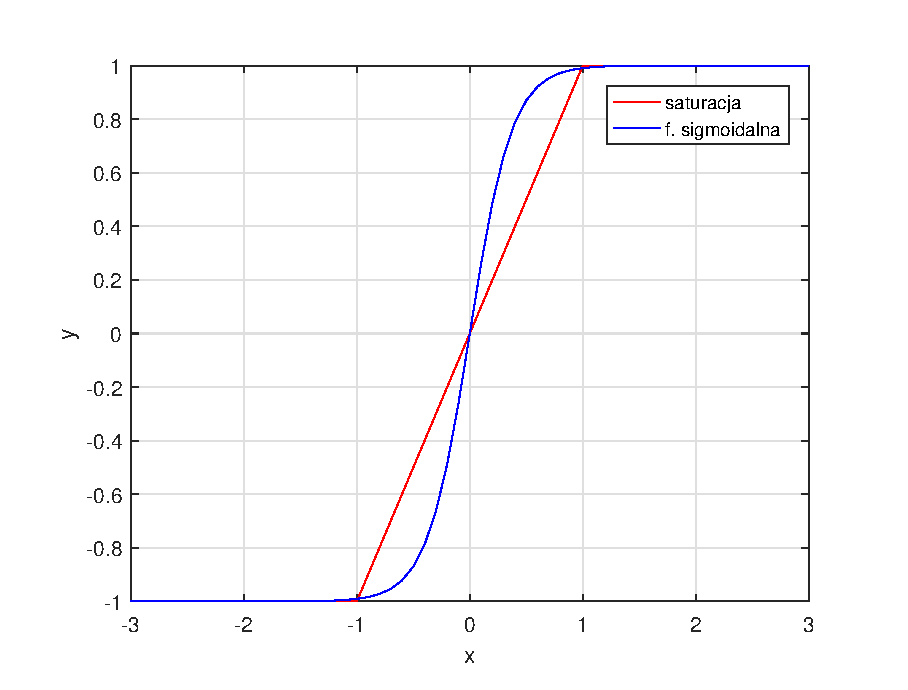
\includegraphics[scale = 0.8]{fig/por_sat_2.eps}
	\caption		
	{Porównanie saturacji i funkcji sigmoidalnej - pusta szklanka.}
	\label{por_sat2}
\end{figure} 

\begin{figure}[h!]
	\centering
	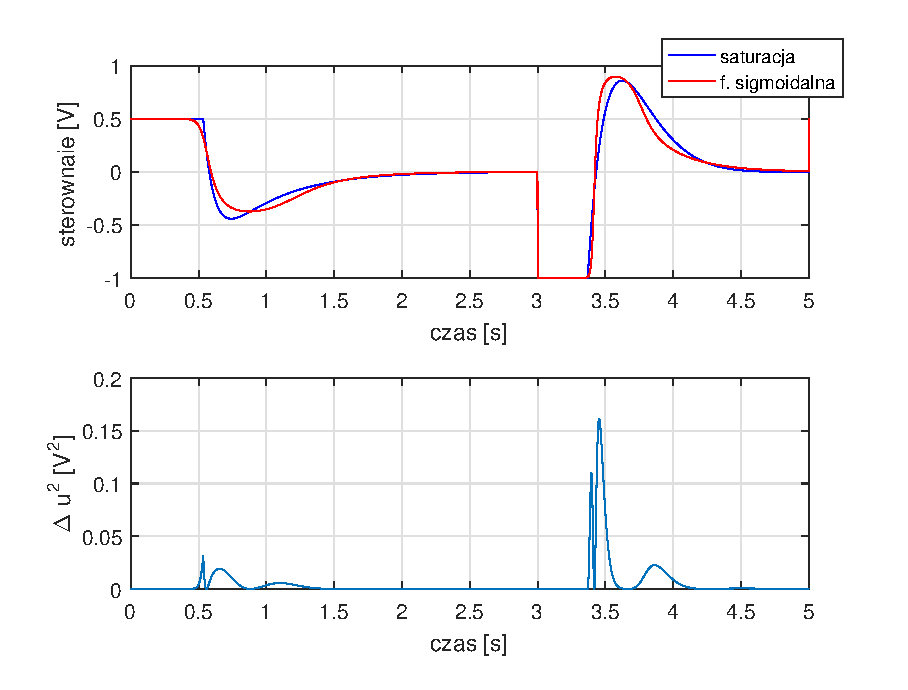
\includegraphics[scale = 1]{fig/por_ster_n.eps}
	\caption		
	{Porównanie sterowania dla regulatora neuronowego.}
	\label{neuron_ster_por}
\end{figure}
\FloatBarrier
\section{Porównanie wska\'zników jakości}
\begin{table}[h]
	\caption{Porównanie wska\'zników jakości regulator PID - neuronowy + saturacja - neuronowy + f. sigmoidalna.}
	\label{por_reg_pid_n_n}
	\centering
	
	\begin{tabular}{|c|M{2.5cm}|M{2.5cm}|M{2.5cm}|}
		\hline
		Regulator [g]&$J_1$&$J_2$&$J_3$\\
		\hline
		PID &3.739&   0.841 &  4.580\\
		\hline
		Neuronowy + saturacja &3.739 &  0.841 &  4.580\\
		\hline
		Neuronowy + f. sigmoidalna & 3.741 &  0.857 &  4.597\\
		\hline
	\end{tabular}
\end{table}